
We apply a PostGIS spatial join query using ST\_WITHIN to select only those
polygons from the segmented dataset that fall completely within the biotope
polygon of our pre-processed biotope map. We join those polygons
with EUNIS characteristics and also attach zonal statistics that are calculated
for every polygon. The last step in the pre-processing workflow is the
replacement of any NULL values with zeros. 
The null values arise due to small polygon sizes created by the segmentation
process. In the future, a new segmented dataset that respects the biotope
boundaries should be available and will reduce the problems from selecting
polygons that fall completely within
% the polygon.
%\begin{figure}
%  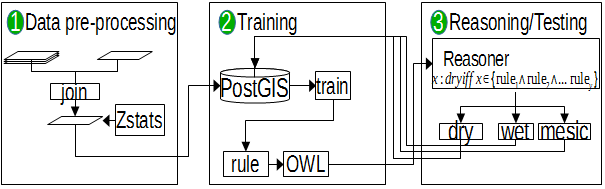
\includegraphics[width=1\linewidth]{diagrams/workflow_overview2.png}
%\caption{A small overview.}
%\end{figure}
The first step was to clip the biotope map with the extent of Saarburg.
Then we join the expert knowledge-derived table that translates the OSIRIS
biotopes to the corresponding EUNIS biotope class. We then perform a spatial
join using PostGIS ST\_WITHIN to select the segmented polygons that lie within
the biotope map. These polygons have all the biotope information
attached to them and in the final step have the zonal statistics with
morphological and hydrological (SAGA wetness index, ) and topographic indices 
(topographic wetness index, ). 
After joining EUNIS characteristics to the RLP
biotope map, the map was spatially joined with the pre-segmented remote sensing
data. software was used for the segmentation and was performed by RLP AgroScience. 
%The remote sensing data already had zonal statistics computed for all of the
%polygons. A list of the zonal statistics are below.
%% INSERT LIST?

\subsection{Ontology-based Reasoning}
Both the data mining algorithms, SEaTH and Decision Trees can produce rule
sets with defined thresholds. The rules can be chained together with logical
operators (AND, OR, NOT) and using a script written in Python, are imported
into an OWL ontology. The polygons from the PostGIS database can be imported
as individuals with their corresponding zonal statistics and other properties
available. Once in an ontology, a reasoner can perform A-Box and T-Box
reasoning. T-Box reasoning allows one to see the relationships between the
EUNIS classes, whereas A-Box reasoning allows the individuals to be classified
into the various defined classes based on the rules imported from the data
mining algorithms. The reasoner also points out logical inconsistencies and
subsumption of concepts in the rules or classes. Identifying logical
inconsistencies can greatly help see how the classes
could be better defined.
We chose Fact++ Reasoner for its speed, efficiency and
capabilities.

\subsection{Semantic-based image interpretation}
Different fields (medical imaging, security, etc.) have used ontologies for
improving image retrieval and object detection. Only recently have ontologies
been adopted in remote sensing research. An ontology, defined as ``an explicit
specification of a conceptualization'' \citep{gruber1993} could help bridge the
semantic gap and allow for better data interoperability, workflow management and
automatic image interpretation \citep{Arvor2013} \citep{Andres2013a}. The term
``semantic gap'' refers to the difference between the higher-level descriptions
by experts and what can be extracted from the visual data. Remote sensing and
field expert knowledge can be digitized in ontologies, thus allowing for a
hierarchy of concepts for improved automatic image annotation and retrieval
using concepts from both fields to produce more accurate results
\citep{Srikanth:2005:EOA:1076034.1076128}. Janowicz \citep{Janowicz2012}
advocates for more observation-driven ontologies and for including machine
learning, geostatistics and data mining to construct ontological primitives.
Research on using observation-based ontologies for classifications is still
lacking. There are initiatives to use ontologies in biodiversity research. Below
are some examples.
\subsection{Ontologies in remote sensing research}

\subsection{Feature selection}
%% focus on ML?
There are many different classification approaches with varying degrees of
complexity and requiring different levels of user input. One commonly used
classification approach, the maximum likelihood classification (MLC) approach,
among the most popular, has been used to study land use change in China-
\citep{Ding2007}, analyze forest cover in Haiti \citep{Churches2014} and land
cover and land-use change in Egypt \citep{Shalaby2007}. Recent research suggests
support vector machines (SVMs) when compared to decision trees (DTs), a neural
network classifier and the MLC, produces better results \citep{Huang2002}. One
such DT is the ``Random Forest'' algorithm which has been shown to be better
than Adaboost \citep{Chan2008} and performed well when applied to the Cape Cod
National Seashore for coastal dune and salt marsh classification
\citep{Timm2012}.
% need more?
\section{State of Research and Research Question}
Remote sensing has a rich history in environmental conservation, meteorology,
climate science and other fields. Due to this history remote sensing experts
have become very good at analyzing remote sensing data. Yet, remote sensing
image analysis implicitly incorporates the expertise and knowledge of the
individual performing the analysis and reduces objectivity. This can be divided
into remote sensing knowledge (spectral signature, remote sensing index, etc.)
and field knowledge (feature properties, spatial relations, etc)
\citep{Andres2013a}. This knowledge is often neither completely nor explicitly
defined but influences the classification. Thus, two experts can interpret the
same image differently due to their unique conceptualizations and experiences.
Further complicating matters, the classification chain is not documented and
controlled, reducing comparability and hindering attempts to reproduce the
results\citep{Arvor2013}. Therefore automated methods for remote sensing
classifications that produce accurate and reproducible results are desired.
An automated system would also reduce the time needed to analyze large
remote sensing datasets. Many approaches have been used to create an accurate
automated classification tool using statistics and different algorithms
from machine learning and data mining. Unfortunately most of these approaches
rely on experts to produce rule-sets or manually select training points. The
former relies on \emph{a priori} knowledge while the latter can be
time-consuming.
Neither are observation-based. There are many different automatic methods
for feature selection. A brief overview explaining the most common methods is
described below.


One of the goals of the projects is
multi-functionality which entails differing semantic conceptualizations. The use
of ontologies and ontology-based reasoning over vector objects was seen as the
solution to this problem. Using ontologies with the help of experts allows for
the translation from the Rhineland-Palatinate biotope system to the EU-wide EU
Nature Information System (EUNIS). Ontologies also allows
for comparison between areas with differing semantic conceptualizations and a
reasoning over objects. 

% dead;
Yet as Lucas et. al (2015) point out there are no standards for classifying
habitats with Earth Observation (EO) data that can be applied to all sites. 

Due to differing standards and approaches of the various nature conservation
agencies in collecting and disseminating information, data comparison is
difficult. Different data types and data sources increase the difficulty in
comparing data from one site to another. Furthermore, habitat monitoring can
be labour intensive and subjective.

Luckily, EO data could help reduce the burden of environmental monitoring and
also provide information on conservation status.
